\documentclass[a4paper,11pt,fleqn]{article}%fleqn pour aligner les equations à gauche
\usepackage{/home/rweye/Nextcloud/Documents/Overleaf/Styles/Eval}

\newcommand{\chnum}{Chapitre 15}
\newcommand{\chtitle}{DS Lumière et spectres}
\newcommand{\dtype}{Evaluation}

\begin{document}
\maketitle
\section*{Question de cours :}
Décrire en vous aidant d’un schéma annoté, une méthode permettant de décomposer la lumière blanche.

\section{Distance Terre-Lune}
Lors des missions lunaires, les astronautes ont déposé des miroirs sur le Lune. Ces miroirs sont utilisés pour déterminer précisément la distance entre la Terre et la Lune. Une mesure a donné pour un aller-retour de la lumière une durée $\Delta t = \SI{2,4282278641}{s}$ avec une précision de $\SI{3E-10}{s}$.
\begin{enumerate}
    \item Schématiser le trajet de la lumière.
    \item \begin{enumerate}
        \item Exprimer la distance $d$ entre la station laser et le miroir visé à la surface de la Lune en fonction de $c$ et de $\Delta t$.
        \item Calculer cette distance $d$ sachant que $c=\SI{299792458}{\meter\per\second}$.
        \item Quelle distance la lumière parcourt-elle en $\SI{3E-10}{s}$ ?
        \item En déduire la précision de la mesure $d$.
    \end{enumerate}
\end{enumerate}

\section{Gaz inconnu}
\begin{multicols}{2}
Voici les longueurs d’onde de quelques radiations émises par le cadmium : \SI{468}{nm}, \SI{480}{nm}, \SI{508}{nm}, \SI{643}{nm}. On a réalisé, à l’aide d’un spectrophotomètre, le spectre de la lumière émise par un gaz. Le spectre est reproduit ci-contre.\\
\textbf{Ce gaz peut-il être le cadmium ? Justifiez.}\\
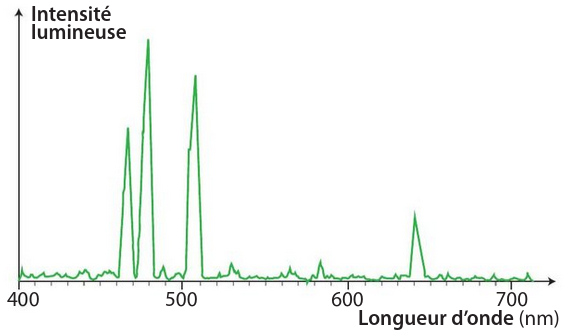
\includegraphics[width =.8\linewidth]{Ressources/2GT_C8_Eval_Fig1.png}

\end{multicols}
\section{Plexiglass}
\begin{minipage}{.5\linewidth}
    On met en place au laboratoire un dispositif utilisant un laser et un hémicylindre pour étudier les phénomènes lumineux. On propose le schéma suivant de l’expérience :
\begin{enumerate}
    \item Définir les différents termes présents sur le schéma : $n_1$, $n_2$, et $i_1$.
    \item Lorsque le rayon lumineux arrive à la surface de l’hémicylindre, quel(s) phénomène(s) physique(s) se met(tent) en place ?
    \item En ce basant sur la réponse précédente et sur les lois de Snell-Descartes, compléter et légender le schéma.
\end{enumerate}
\end{minipage}
\begin{minipage}{.5\linewidth}
\begin{tikzpicture}[scale=.8,transform shape]
    \draw[thick](-4,0) --(4,0);
    \draw[thick,dashed] (0,-4) -- (0,5);
    \draw[thick] (3.36,-4) -- (0,0);
    \draw[thick] (4,0) arc(0:180:4);
    \node (n1) at (4,-1){$n_1 = 1$};
    \node (n2) at (2,1){$n_2 = 1,43$};
    \draw[thick] (0,-.5) arc(270:310:.5);
    \node (i1) at (.75,-2){$i_1 = \SI{40}{\degree}$};
\end{tikzpicture}
\end{minipage}

\section{Ryujin}
On retrouve un échantillon d’eau de mer dont on souhaite déterminer l’origine. On sait que l’indice de réfraction de l’eau salée varie selon la concentration en sel. On dispose de quelques documents ainsi que d’une expérience réalisée avec l’échantillon, schématisée ci-dessous.\\
\textbf{De quelle(s) région(s) du monde peu(ven)t venir cet échantillon ?}\\

\begin{center}
    \begin{tikzpicture}[scale=1.3,transform shape]
    \draw[thick](-4,0) --(4,0);
    \draw[thick,dashed] (0,-4) -- (0,4);
    
    \draw[thick] (-2.31,4) -- (0,0);
    \draw[thick] (0,1) arc(90:120:1);
    \node (i1) at (-.75,3){$i_1 = \SI{30}{\degree}$};
    
    \node (n1) at (3,1){$n_{air}$};
    \node (n2) at (3,-1){$n_{\text{eau salée}}$};

    \draw[thick] (1.42,-4) -- (0,0);
    \draw[thick] (0,-1) arc(270:289.5:1);
    \node (i2) at (.25,-2){$i_2$};
\end{tikzpicture}
\end{center}



\noindent \begin{minipage}{.4\linewidth}
\begin{tabular}{|c|c|}
    \hline \textbf{Mer considérée} & \textbf{Salinité} (en \unit{\gram\per\liter})\\
    \hline Mer Baltique & 3,00 - 8,00\\
    \hline Mer Noire & 18,3 - 22,2\\
    \hline Océan Atlantique & 33,5 - 37,4 \\
    \hline Océan Pacifique & 34,5 - 36,9 \\
    \hline Océan Indien & 35,5 - 36,7\\
    \hline Mer Méditerranée & 38,4 - 41,2 \\
    \hline Mer Rouge & 50,8 - 58,5\\
    \hline Mer Morte & 192,2 - 260\\
    \hline
\end{tabular}
\end{minipage}
\hspace{1em}
\begin{minipage}{.6\linewidth}
\begin{tikzpicture}
    \draw[-Stealth] (0,0) to (8.5,0);
    \draw[-Stealth] (0,0) to (0,6.5);
    \foreach \k in {0,1,...,8}{
        \pgfmathsetmacro\x{10*\k}
        \draw (\k,-.1)--(\k,.1);
        \draw (\k,0) node[below]{\pgfmathprintnumber[precision=1]{\x}};
        }
    \foreach \d in {0,1,...,6} {
        \pgfmathsetmacro\y{13.3+0.05*\d}
        \pgfkeys{/pgf/number format/.cd,fixed,fixed zerofill,precision=2}
        \draw (-.1,\d)--(.1,\d);
        \draw (0,\d) node[left]{\pgfmathprintnumber[precision=2]{\y}};
        \draw[gray] (-.1,\d)--(8,\d);
        }
    \draw(0,0.272)-- (7,4.892);
    \node (x) at (4,-1){Concentration en masse de sel (en \unit{\gram\per\liter})};
    \node[rotate =90] (y) at (-1.5,3){Indice de réfraction de l'eau salée};
\end{tikzpicture}
\end{minipage}
\end{document}